\documentclass[crop,tikz,border=10px,convert=pdf2svg,multi=false]{standalone}
\usepackage{amsfonts}
\usepackage[defaultsans]{opensans}
\usetikzlibrary{shapes,arrows,positioning}
\begin{document}
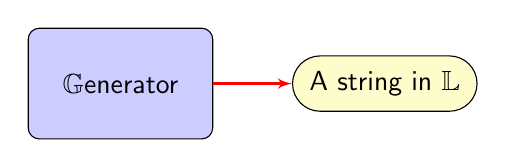
\begin{tikzpicture}[font=\sffamily,
  block/.style = {rectangle, draw, fill=blue!20, text centered, text
    width=6em, rounded corners, minimum height=4em},
  cloud/.style = {rectangle, draw, fill=yellow!20, text centered, text
    width=6em, rounded corners=10pt, minimum height=2em},
  line/.style = {-latex', red, thick},
  legend/.style = {draw=none, font=\sffamily, text centered}]

  \node[block] (generator) {\(\mathbb{G}\)enerator};
  \node[cloud, right=of generator] (output) {A string in \(\mathbb{L}\)};

  \draw [line] (generator) -- (output);

\end{tikzpicture}
\end{document}
